\chapter*{Introduction}
\addcontentsline{toc}{chapter}{Introduction}

\par Free surface fluid flows and processes involved in a fluid behavior fascinated scientists since the very beginning of the scientific history. Problems as a breakup of a liquid jet, droplet formation and merging, rising bubbles etc. still lacks deeper understanding because of a complex and nonlinear equations governing such phenomena. In addition, they play a role in many industrial processes: \textit{fuel injection, fibre spinning, ink-jet printing etc.} EGGERS

\par The equations for the motion of a fluid formulated in the 19th century came to relevance as computers started to provide number of numerical methods for finding their approximate solutions. However, majority of the methods are well suited for problems involving one-phase flows or fluid-wall interactions, multi-phase flows, fluid-fluid interactions, surface forces and similar issues still remain debated and incomplete.

\par Imagine some usual situation, where a water droplet hanging on a tap is being pulled down by the gravity. From a physical point of view, the behavior and evolution is well described. \textit{Navier-Stokes} equations govern the fluid motion in each phase, water and air separately, while discrete surface forces(surface tension) are balanced with the gravitational, volume force. Mathematically, not only an existence and uniqueness of a solution of the equations was proven, but multiple domains coupled with complex boundary conditions must be taken into account.


\begin{figure}[ht]
\centering
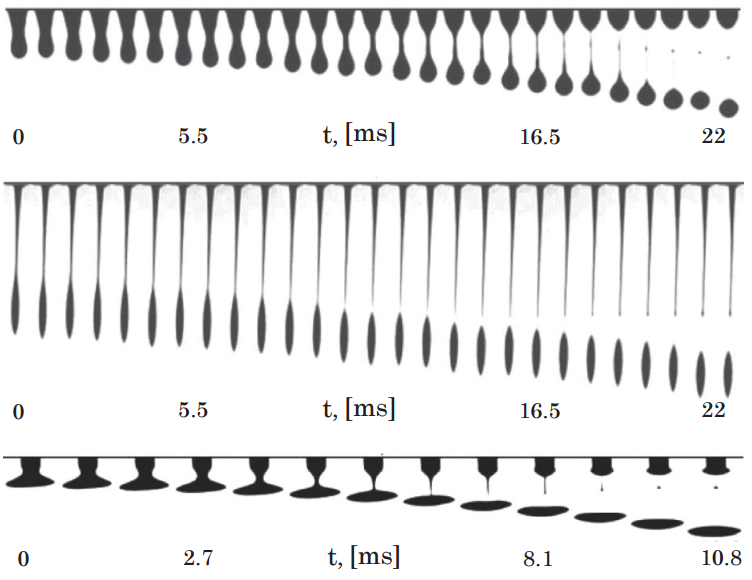
\includegraphics[width=80mm]{img/ferrofluid_motivation.png}
\caption{High-speed image sequence of ferrofluid droplet dripping out of a container. Influence of a magnetic field parallel(middle) and perpendicular(bottom) to the direction of the flow is clearly visible. Taken from [HABERA]}
\end{figure}

\par All these phenomena become even more attractive in terms of \textit{ferrohydrodynamics}. Ferrofluid reacts to magnetic field and changes its shape due to an additional surface force. This entirely changes dynamics of the droplet formation process and it will be the object for our studies.

\par In the first part of the thesis a brief summary of the physical and mathematical model and numerical methods are given. Navier-Stokes equations are solved using the \textit{projection methods} and spatially approximated in sense of weak derivates and \textit{finite element method}. Interface is represented with the \textit{level-set} function, while the conservation of its volume is assured with the reinitialization step.  

\par In the second part we discuss the results of the implemented methods and give a direct comparison of our results with experimental data obtained in HABERA.
